\documentclass{article}
\usepackage{../m}
\usepackage{graphicx}

\begin{document}
\noindent Paul Gustafson\\
\noindent Texas A\&M University - Math 641\\ 
\noindent Instructor - Fran Narcowich

\subsection*{Final}
\p{1} Let $f \in C[0,2 \pi]$ with $f(0) = f(2\pi)$.  Let 
$Q_{trap}(f) =  \frac {2\pi} n \sum_{k=0}^{n-1} f \left(\frac {2 \pi k} n \right)$.
Let $E_n = \left| \int_0^{2 \pi} f(x) dx - Q_n(f) \right|$.

\begin{enumerate}[(a)]
\item Show $Q_{trap}(e^{ikx}) = \left\{ 
\begin{array}{ll}
0 & k \not\equiv 0 \pmod n
\\ 2\pi & k \equiv 0 \pmod n
\end{array}
\right.$

\begin{proof}
If $k \equiv 0 \pmod n$, we have $Q_{trap} = \frac {2\pi} n \sum_{j=0}^{n-1} e^{\frac {2 \pi i jk} n} = \frac{2 \pi}{n} \sum_{j=0}^{n-1} 1 = 2\pi$.

Otherwise, we have 
\begin{align*}
Q_{trap}(e^{ikx}) & = \frac {2\pi} n \sum_{j=0}^{n-1} e^{\frac {2 \pi i jk} n}
\\ & = \frac {2\pi} n \frac{1 -  e^{2 \pi i k}}{1 - e^{\frac {2 \pi i k} n}}
\\ & = 0
\end{align*}
\end{proof}

\item Let $f(x)$ be the $2 \pi$-periodic function that equals $x^2(2\pi - x)^2$ when $x \in [0, 2\pi]$. Show that $\int_0^{2\pi} f(x) dx = 16 \pi^5/15$. Prove that $E_n \le C n^{-4}$.  
(Hint: $f(x) = \frac{8\pi^4}{15} - \frac{24}{\pi} \sum_{k \neq 0} e^{ikx} k^{-4}$.)

\begin{proof}
We have
\begin{align*}
\int_0^{2 \pi} x^2(2\pi - x)^2 dx & = \int_0^{2 \pi} 4\pi^2 x^2 - 4 \pi x^3 + x^4 \, dx
\\ & = \frac 4 3 \pi^2 (2\pi)^3 - \pi(2 \pi)^4 + \frac 1 5 (2 \pi)^5
\\ & = \frac 4 3 \pi^2 (2\pi)^3 - \pi(2 \pi)^4 + \frac 1 5 (2 \pi)^5
\\ & = (32 \cdot 5 - 16 \cdot 15 + 32 \cdot 3) \pi^5/15
\\ & = 16 \pi^5/15
\end{align*}

On the midterm we calculated the Fourier expansion for $f$, so I will assume the hint without proof. Thus
\begin{align*}
E_n & = | \frac {16 \pi^5}{15} - Q_n(\frac{8\pi^4}{15} - \frac{24}{\pi} \sum_{k \ge 0 } e^{ikx} k^{-4}) |
\\ & =  | \frac C n \sum_{j=0}^{n-1} \sum_{k \ge 0} e^{2\pi ikj/n} k^{-4}) |
\\ & = | \frac C n \sum_{k \ge 0} k^{-4} \sum_{j=0}^{n-1} e^{2\pi ikj/n} |
\\ & = C' \sum_{k \ge 0} k^{-4} Q_n(e^{ikx})
\\ & = C' \sum_{k \ge 0} 2 \pi (nk)^{-4}
\\ & = C'' n^{-4}
\end{align*}
where the interchange of summation is justified by the absolute summability of the series.
\end{proof}

\item Use Matlab or some other program to plot $\log(E_n)$ vs. $\log n$ for $n = 16, 24, 256, 1024$. This should be a straight line. What is its slope? Does it agree with what you found in (b)?

\begin{proof}


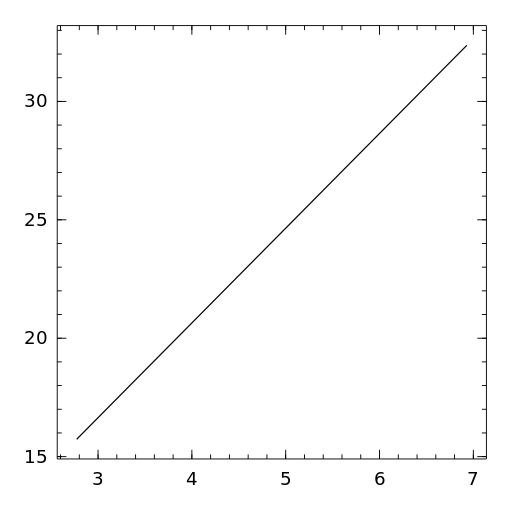
\includegraphics[width=2in]{lognVlogE.png}

The above plots $\log n$ on the $x$-axis and $\log E_n$ on the $y$-axis. The slope according to (b) should be $-4$. The graph seems to agree.
\end{proof}

\end{enumerate}

\p 2 Let $\mH$ be a complex Hilbert space, and let $L \in \mB(\mH)$.
\begin{enumerate}
\item Verify that 
$\langle L(u + e^{i \alpha} v), u + e^{i \alpha} v \rangle - 
\langle L(u - e^{i \alpha} v), u - e^{i \alpha} v \rangle
= 2 e^{-i \alpha} \langle L u, v \rangle + 2 e^{-i \alpha} \langle Lv, u \rangle$

\begin{proof}
We have 
\begin{align*}
\langle L(u + e^{i \alpha} v), u + e^{i \alpha} v \rangle - 
\langle L(u - e^{i \alpha} v), u - e^{i \alpha} v \rangle
& = \langle Lu, u \rangle + \langle Lu, e^{i \alpha} v \rangle +
\langle e^{i \alpha} v), u \rangle + \langle u, v \rangle
\\ & \quad - \langle Lu, u \rangle + \langle Lu, e^{i \alpha} v \rangle +
\langle e^{i \alpha} v), u \rangle - \langle u, v \rangle
\\ & = 2 e^{-i \alpha} \langle L u, v \rangle + 2 e^{-i \alpha} \langle Lv, u \rangle
\end{align*}
\end{proof}

\item Show that if $L = L^*$, then $\|L \| = \sup_{\|u\| = 1} | \langle L u, u \rangle |$.

\begin{proof}
Acknowledgement: I looked at  http://www.math.washington.edu/~hart/m556/lecture2.pdf for hints.

By Cauchy-Schwarz, we have $\sup_{\|u\| = 1} | \langle L u, u \rangle | \le 
\sup_{\|u\| = 1} \|L u\| = \|L \|$.

For the reverse inequality, recall from a previous homework problem that $\|L\| = \sup_{\|u\| = 1, \|v\| = 1} |\langle L u, v \rangle\|$.
Pick $(u_n), (v_n)$ such that $|\langle Lu_n, v_n \rangle | \to \|L\|$.  Pick $\alpha_n \in [0, 2\pi]$ such that 
$e^{i\alpha_n} \langle Lu_n, v_n \rangle = |\langle Lu_n, v_n \rangle |$. Let $w_n = e^{-i\alpha_n} v_n$. Thus, $\langle Lu_n, w_n \rangle \to \|L\|$.
In particular, $\|L\| \le  \sup_{\|u\| = 1, \|v\| = 1} \Re \langle Lu, v \rangle$. Since $\Re \langle Lu, v \rangle \le |\langle Lu, v \rangle|$, we have $\|L\| = \sup_{\|u\| = 1, \|v\| = 1} \Re \langle Lu, v \rangle$.

For $\|u\| = \|v\| = 1$, we have
\begin{align*}
\Re \langle Lu, v \rangle & =  \frac 1 2 (\langle Lu, v \rangle + \langle v, Lu \rangle)
\\ & = \frac 1 2 (\langle Lu, v \rangle + \langle Lv, u \rangle)
\\ & = \frac 1 4  (\langle L(u + v), u + v\rangle -  \langle L(u - v), u - v \rangle)
\\ &  \le \frac 1 4 ( \|u + v\|^2 + \|u - v\|^2) \sup_{\|u\| = 1} | \langle L u, u \rangle |
\\ &  \le \frac 1 2 ( \|u\|^2 + \|v\|^2) \sup_{\|u\| = 1} | \langle L u, u \rangle |
\\ &  \le \frac 1 2 ( \|u\|^2 + \|v\|^2) \sup_{\|u\| = 1} | \langle L u, u \rangle |
\\ &  = \sup_{\|u\| = 1} | \langle L u, u \rangle |
\end{align*}
\end{proof}

\item Show that if $M = \sup_{\|u\| = 1} |\langle Lu, u \rangle|$, then $M \le \|L\| \le 2M$, whether or not $L$ is self-adjoint. Give an example that shows that this result is false in a real Hilbert space.


\begin{proof}
By Cauchy-Schwarz, we have $M = \sup_{\|u\| = 1} | \langle L u, u \rangle | \le 
\sup_{\|u\| = 1} \|L u\| = \|L \|$.

For the other inequality,  let $\|u\| = \|v\| = 1$ and $\alpha \in \R$.  By part (a),
\begin{align*}
\Re \langle Lu, v \rangle | &  = \frac 1 2 \Re( \langle L(u + e^{i \alpha} v), u + e^{i \alpha} v \rangle - 
\langle L(u - e^{i \alpha} v), u - e^{i \alpha} v \rangle
- 2 e^{-i \alpha} \langle Lv, u \rangle )
\\ & \le \frac  M 2 ( \|u + e^{i \alpha} v\|^2 + \|u - e^{i \alpha} v \|^2)  - \Re ( 2 e^{-i \alpha} \langle Lv, u \rangle )
\\ & =   M ( \|u\|^2 + \|e^{i \alpha} v \|^2)  - \Re ( 2 e^{-i \alpha} \langle Lv, u \rangle )
\\ & = 2 M  - \Re ( 2 e^{-i \alpha} \langle Lv, u \rangle )
\end{align*}
By picking $\alpha$ appropriately, we can ensure that $e^{-i \alpha} \langle Lv, u \rangle$ is a nonnegative real number.  Thus $\Re \langle Lu, v \rangle | \le 2M$.  Thus, $\|L\| \le 2M$.


For the counterexample in the real case, let $\mH = \R^2$ with the standard inner product.  Let 
$$L = \begin{pmatrix}
0 & 1
\\ -1  & 0
\end{pmatrix}$$.
Then $\langle Lu, u\rangle = 0$ for all $u$, but $\|L\| = 1$.
\end{proof}
\end{enumerate}

\p 3 Let $K \in \mC(\mH)$ be self adjoint. Show that the only possible limit point of the set of eigenvalues of $K$ is 0.
\begin{proof}
Let $\epsilon > 0$. Let $\mE_\lambda$ be the eigenspace corresponding to an eigenvector $\lambda$.  Let $X = \bigoplus_{|\lambda| > \epsilon} \mE_\lambda$. Then $X$ is an invariant subspace for $K$, and $K$ maps the unit ball $B_X$ of $X$ to a precompact set. Moreover $\epsilon B_X \subset K B_x$. But this implies that $B_X$ is precompact.  Hence $X$ must be finite-dimensional, so there can only be finitely many $\lambda$ with $|\lambda| > \epsilon$.
\end{proof}


\p 4 Let $K \in \mC(\mH)$ be self adjoint. Suppose the range of $K$ contains a dense subset of $\mH$, and that an o.n. basis has been chosen for the igenspace of each nonzero eigenvalue of $K$. Show that the set of all these eigenvectors form a complete orthormal set.
\begin{proof}
By a theorem in class, we know that this set (call it $S$) is orthogonal. Thus we only need to show that the span of $S$ is dense in $\mH$. The spectral theorem states that an o.n. basis $B$ of eigenvectors for $K$ exists. We can write each vector in $B$ as a sum of vectors in $S$ since $S$ spans each eigenspace.  Thus, $\spn S = \spn B = \mH$.
\end{proof}


\p 5 Let $\mH = L^2[0,1]$. Consider the boundary value problem
$$Lu := \frac d {dx} \left( (1 + x) \frac {du} {dx} \right) = f(x),
u(0) = 0, u'(1) = 0.$$

\begin{enumerate}[(a)]
\item Find $G(x,y)$, the Green's function for this BVP.

\begin{proof}
The fundamental set for this BVP is $\{1, \log(1 + x)\}$.
The Wronskian of these two functions is $W(x) = \log(1+x)$. 
Hence, the Green's function is
$$G(x,y) = \left\{ \begin{array}{ll}
\frac {\log(1+x)}{\log(1 + y)}, & \text{ if } 0 \le x \le y \le 1
\\\frac {\log(1+y)}{\log(1 + x)}, & \text{ if } 0 \le y \le x \le 1
\end{array}
\right.
$$
\end{proof}
\item Let $Gf(x) = \int_0^1 G(x,y) f(y) dy$. Show that the range of $G$ contains a dense set in $\mH$. 
\begin{proof}
Let $S$ be the set of $u \in C^2[0,1]$ with support in $(0,1)$.  Note that if $u \in S$ then $u$ satisfies the boundary conditions of the BVP.  Hence, we can just plug $u$ into the differential equation to find $f$ such that $Gf = u$.  Thus the range of $G$ contains $S$.

To see that $S$ is dense in $\mH$, recall that functions of the form $g(x) = e^{inx}$ form a basis for $L^2[0,1]$.  Thus, it suffices to approximate $g(x) = e^{inx}$ by elements of $S$ in the $L^2$ norm. Letting $\epsilon > 0$, we can cut off the $[0, \epsilon/4)$ and $(1- \epsilon/4, 1]$ ends off $g$ and replace them with a $C^2$ spline on each end which agree up to second derivatives with $g$ at $\epsilon/4$ and $1 - \epsilon/4$.  Moreover, we can ensure that the splines are $0$ near $0$ and $1$, respectively, and have sup-norm $2$. This new function $h$ is in $S$ and $\|g - h\|_{L^2} < \epsilon$.
\end{proof}

\item Use it and the previous problem to show that the eigenfunctions for $\frac d {dx} \left((1+x) \frac{du}{dx}\right) + \lambda u = 0, u(0) = 0, u'(1) = 0$ form a complete orthogonal set.
\begin{proof}
The the function $G(x,y)$ is bounded hence $L^2$. Thus, the operator $G$ is Hilbert-Schmidt hence compact.  Moreover, $G(x,y)$ is symmetric so $G$ is self-adjoint.  Thus we can apply part (b) and problem (4) to get that the eigenfunctions form a complete orthogonal set.
\end{proof}
\end{enumerate}

\p 6 Let $\| \cdot \|_{op}$ be the operator norm for $\mB(\mH)$.
\begin{enumerate}
\item Show that $(\mB(\mH), \|\cdot \|_{op})$ is a Banach space.
\begin{proof}
We need to show that $\| \cdot \|_{op}$ is positive definite, homogeneous, and satisfies the triangle inequality.  

It is clearly positive. Moreover, if $\|T\|_{op} = 0$, then $\|Tu\| = 0$ for all $\|u\| = 1$.  Hence $Tv = \|v\| T \frac v {\|v\|} = 0$ for all $v \in \mH \setminus \{0\}$.  Thus $Tv = 0$.

For the homogeneity, we have $\|cT\|_{op} = \sup_{\|u\| = 1} |c|\|Tu\| = |c| \|T\|_{op}$ for all $c \in \R$ and $T \in \mH$.

For the triangle inequality, we have 
$\|S + T \|_{op} = \sup_{\|u\|=1} \|Su + Tu\| \le \sup_{\|u\|=1} \|Su \| + \|Tu\| 
\le \sup_{\|u\|=1} \|Su \| + \sup_{\|v\| = 1} \|Tv\|  = \|S\|_{op} + \|T\|_{op}$.
\end{proof}

\item Consider the operator $L = I - \lambda M$, with $M \in \mB(\mH)$. Show that if $|\lambda| < \|M \|_{op}^{-1}$, then, in the operator norm,
$\sum_{k=0}^\infty \lambda^k M^k = (I - \lambda M)^{-1}$.

\begin{proof}
First note that $\|(I - \overline \lambda M^*)u\| \ge \|u\| - \|\overline \lambda M^* u\| > 0$ for all $u \neq 0$.  Thus, $\mN(I - \overline \lambda M^*) = \{0\}$ so $L$ is invertible by the Fredholm Alternative theorem.

For $\|u\| = 1$, write $u = (I - \lambda M)v$. Then
\begin{align*}
((I - \lambda M)^{-1} - \sum_{k=0}^K \lambda^k M^k) u & = v - \sum_{k=0}^K \lambda^k M^k (I - \lambda M)v
\\ & = v - \sum_{k=0}^K \lambda^k M^k +  \sum_{k=0}^K \lambda^{k+1} M^{k+1} v
\\ & = v - \sum_{k=0}^K \lambda^k M^k +  \sum_{k=0}^K \lambda^{k+1} M^{k+1} v
\\ & = \lambda^{k+1} M^{k+1} v
\\ & \le \lambda^{k+1} M^{k+1} \|(I - \lambda M)^{-1}\|
\\ & \to 0
\end{align*}
as $k \to \infty$. Since the last estimate is uniform in $u$, the converge holds in the operator norm.
\end{proof}

\end{enumerate}

\p 7 Show that if $B, B^{-1}$ are in $\mB(\mH)$, and $K \in \mC(\mH)$, then the range of $L = B + \lambda K$ is closed.

\begin{proof}
Suppose $Lx_n \to y$. We need to find $x$ such that $Lx = y$. By passing to a subsequence, since $\lambda K$ is compact, we may assume $\lambda K x_n \to z$.  Then $B x_n \to y - z$.   Since $B^{-1}$ is continuous, we have $x_n \to B^{-1}(y-z)$. 

Let $x = B^{-1}(y-z)$. Then $Lx = L B^{-1}(y-z) = (y - z) + \lambda K B^{-1}(y-z) =  (y - z) + \lambda K \lim_n x_n = y$.
\end{proof}

\end{document}











